% !TeX root = ./0_article.tex

\section{Logic path under BBI}
For the purpose of analyzing the effects og BBI on actual logic, this section is dedicated in modeling and simulating an actual logic path
In this section, we are lingering on analyzing the effects of BBI on more complex logic paths.
The study is conducted for both a static logic path and a dynamic logic path.
The considered logic paths are constituted of inverters, buffers and a D-Flip-Flop (DFF).
The inverters model an arbitrary combinatorial logic path tackling the input of a DFF, used to sample the logic path output.
The DFF clock is buffered to achieve an isolation from the ideal voltage source.
Then, the DFF output is injected into a final 4-IVX chain, loaded with a 5 pF capacitor.
The resulting schematic is described in Fig. \ref{dffChain}.

\begin{figure}[h]
	\label{dffChain}
	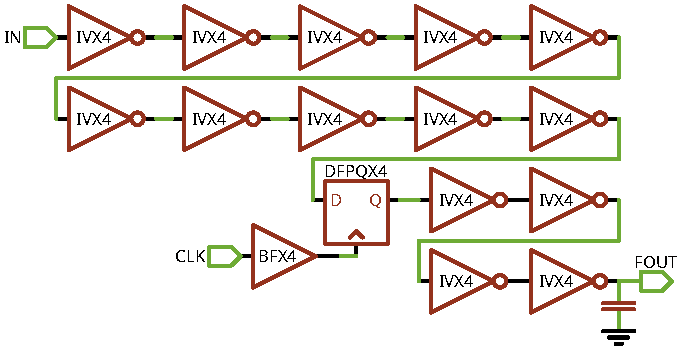
\includegraphics[width=0.5\textwidth]{./figures/dff_ivx_chain_2.pdf}
	\caption{DFFCHAIN}
\end{figure}
